\section{15. Multivariate Models}\label{multivariate-models}

Review of notation from linear algebra:

\begin{itemize}[tightlist]
\item
  If \(x\) and \(y\) are vectors, then \(x^T y = \sum_j x_j y_j\).
\item
  If \(A\) is a matrix then \(\text{det}(A)\) denotes the determinant of
  \(A\), \(A^T\) denotes the transpose of A, and \(A^{-1}\) denotes the
  inverse of \(A\) (if the inverse exists).
\item
  The trace of a square matrix \(A\), denoted by \(\text{tr}(A)\), is
  the sum of its diagonal elements.
\item
  The trace satisfies \(\text{tr}(AB) = \text{tr}(BA)\) and
  \(\text{tr}(A + B) = \text{tr}(A) + \text{tr}(B)\).
\item
  The trace satisfies \(\text{tr}(a) = a\) if \(a\) is a scalar.
\item
  A matrix \(\Sigma\) is positive definite if \(x^T \Sigma x > 0\) for
  all non-zero vectors \(x\).
\item
  If a matrix \(\Sigma\) is symmetric and positive definite, there
  exists a matrix \(\Sigma^{1/2}\), called the square root of
  \(\Sigma\), with the following properties:

  \begin{itemize}[tightlist]
  \item
\(\Sigma^{1/2}\) is symmetric
  \item
\(\Sigma = \Sigma^{1/2} \Sigma^{1/2}\)
  \item
\(\Sigma^{1/2} \Sigma^{-1/2} = \Sigma^{-1/2} \Sigma^{1/2} = I\)
    where \(\Sigma^{-1/2} = (\Sigma^{1/2})^{-1}\).
  \end{itemize}
\end{itemize}

\subsection{15.1 Random Vectors}\label{random-vectors}

    Multivariate models involve a random vector \(X\) of the form

\[X = \begin{pmatrix} X_1 \\ \vdots \\ X_k \end{pmatrix}\]

The mean of a random vector \(X\) is defined by

\[\mu 
= \begin{pmatrix} \mu_1 \\ \vdots \\ mu_k \end{pmatrix} 
= \begin{pmatrix} \mathbb{E}(X_1) \\ \vdots \\ \mathbb{E}(X_k) \end{pmatrix}
\]

The covariance matrix \(\Sigma\) is defined to be

\[\Sigma = \mathbb{V}(X) = \begin{pmatrix}
\mathbb{V}(X_1) & \text{Cov}(X_1, X_2) & \cdots & \text{Cov}(X_1, X_k) \\
\text{Cov}(X_2, X_1) & \mathbb{V}(X_2) & \cdots & \text{Cov}(X_2, X_k) \\
\vdots & \vdots & \ddots & \vdots \\
\text{Cov}(X_k, X_1) & \text{Cov}(X_k, X_2) & \cdots & \mathbb{V}(X_k)
\end{pmatrix}\]

This is also called the variance matrix or the variance-covariance
matrix.

\textbf{Theorem 15.1}. Let \(a\) be a vector of length \(k\) and let
\(X\) be a random vector of the same length with mean \(\mu\) and
variance \(\Sigma\). Then \(\mathbb{E}(a^T X) = a^T\mu\) and
\(\mathbb{V}(a^T X) = a^T \Sigma a\). If \(A\) is a matrix with \(k\)
columns then \(\mathbb{E}(AX) = A\mu\) and
\(\mathbb{V}(AX) = A \Sigma A^T\).

Now suppose we have a random sample of \(n\) vectors:

\[
\begin{pmatrix}X_{11} \\ X_{21} \\ \vdots \\ X_{k1} \end{pmatrix}, \;
\begin{pmatrix}X_{21} \\ X_{22} \\ \vdots \\ X_{k2} \end{pmatrix}, \;
\cdots , \;
\begin{pmatrix}X_{1n} \\ X_{2n} \\ \vdots \\ X_{kn} \end{pmatrix}
\]

The sample mean \(\overline{X}\) is a vector defined by

\[\overline{X} = \begin{pmatrix} \overline{X}_1 \\ \vdots \\ \overline{X}_k \end{pmatrix}\]

where \(\overline{X}_i = n^{-1} \sum_{j = 1}^n X_{ij}\). The sample
variance matrix is

\[ S = \begin{pmatrix} 
s_{11} & s_{12} & \cdots & s_{1k} \\
s_{12} & s_{22} & \cdots & s_{2k} \\
\vdots & \vdots & \ddots & \vdots \\
s_{1k} & s_{2k} & \cdots & s_{kk}
\end{pmatrix} \]

where

\[s_{ab} = \frac{1}{n - 1} \sum_{j = 1}^n (X_{aj} - \overline{X}_a) (X_{bj} - \overline{X}_b)\]

It follows that \(\mathbb{E}(\overline{X}) = \mu\) and
\(\mathbb{E}(S) = \Sigma\).

\subsection{15.2 Estimating the
Correlation}\label{estimating-the-correlation}

Consider \(n\) data points from a bivariate distribution

\[
\begin{pmatrix} X_{11} \\ X_{21}\end{pmatrix}, \;
\begin{pmatrix} X_{12} \\ X_{22}\end{pmatrix}, \;
\cdots \;
\begin{pmatrix} X_{1n} \\ X_{1n}\end{pmatrix}
\]

Recall that the correlation between \(X_1\) and \(X_2\) is

\[\rho = \frac{\mathbb{E}((X_1 - \mu) (X_2 - \mu_2))}{\sigma_1 \sigma_2}\]

The sample correlation (the plug-in estimator) is

\[\hat{\rho} = \frac{\sum_{i=1}^n (X_{1i} - \overline{X}_1)(X_{2i} - \overline{X}_2)}{s_1 s_2}\]

We can construct a confidence interval for \(\rho\) by applying the
delta method as usual. However, it turns out that we get a more accurate
confidence interval by first constructing a confidence interval for a
function \(\theta = f(\rho)\) and then applying the inverse function
\(f^{-1}\). The method, due to Fisher, is as follows. Define

\[f(r) = \frac{1}{2} \left( \log(1 + r) - \log(1 - r)\right) \]

and let \(\theta = f(\rho)\). The inverse of \(f\) is

\[g(z) \equiv f^{-1}(z) = \frac{e^{2z} - 1}{e^{2z} + 1}\]

Now do the following steps:

\textbf{Approximate Confidence Interval for the Correlation}

\begin{enumerate}[tightlist,label={\arabic*.}]
\item
  Compute
\end{enumerate}

\[\hat{\theta} = f(\hat{\rho}) = \frac{1}{2} \left( \log(1 + \hat{\rho}) - \log(1 - \hat{\rho})\right) \]

\begin{enumerate}[tightlist,label={\arabic*.},resume]
\item
  Compute the approximate standard error of \(\hat{\theta}\) which can
  be shown to be
\end{enumerate}

\[\hat{\text{se}}(\hat{\theta}) = \frac{1}{\sqrt{n - 3}} \]

\begin{enumerate}[tightlist,label={\arabic*.},resume]
\item
  An approximate \(1 - \alpha\) confidence interval for
  \(\theta = f(\rho)\) is
\end{enumerate}

\[(a, b) \equiv \left(\hat{\theta} - \frac{z_{\alpha/2}}{\sqrt{n - 3}}, \; \hat{\theta} + \frac{z_{\alpha/2}}{\sqrt{n - 3}} \right)\]

\begin{enumerate}[tightlist,label={\arabic*.},resume]
\item
  Apply the inverse transformation \(f^{-1}(z)\) to get a confidence
  interval for \(\rho\):
\end{enumerate}

\[ \left( \frac{e^{2a} - 1}{e^{2a} + 1}, \frac{e^{2b} - 1}{e^{2b} + 1} \right) \]

\subsection{15.3 Multinomial}\label{multinomial}

Review of Multinomial distribution: consider drawing a ball from an urn
that has \(n\) balls of \(k\) colors. Let \(p = (p_1, \dots, p_k)\)
where \(p_j \geq 0\) are the probabilities of drawing (with replacement)
a ball of each color; \(\sum_j p_j = 1\). Draw \(n\) times and let
\(X = (X_1, \dots, X_n)\) where \(X_j\) is the number of times that
color \(j\) appeared; so \(\sum_k X_k = n\). We say \(X\) has a
Multinomial(\(n\), \(p\)) distribution. The probability function is

\[ f(x; p) = \binom{n}{x_1 \dots x_k} p_1^{x_1}\dots p_k^{x_k}\]

where

\[ \binom{n}{x_1 \dots x_k} = \frac{n!}{x_1! \dots x_k!} \]

\textbf{Theorem 15.2}. Let \(X \sim \text{Multinomial}(n, p)\). Then the
marginal distribution of \(X_j\) is
\(X_j \sim \text{Binomial}(n, p_j)\). The mean and variance of \(X\) are

\[\mathbb{E}(X) = \begin{pmatrix} np_1 \\ \vdots \\ np_k \end{pmatrix}\]

and

\[\mathbb{V}(X) = \begin{pmatrix}
np_1(1 - p_1) & -np_1p_2 & \cdots & -np_1p_k \\
-np_1p_2 & np_2(1 - p_2) & \cdots & -np_2p_k \\
\vdots & \vdots & \ddots & \vdots \\
-np_1p_k & -np_2p_k & \cdots & -np_k(1 - p_k)
\end{pmatrix}\]

\textbf{Proof}. That \(X_j \sim \text{Bimomial}(n, p_j)\) follows
easily. Hence \(\mathbb{E}(X_j) = np_j\) and
\(\mathbb{V}(X_j) = np_j(1 - p_j)\).

To compute \(\text{Cov}(X_i, X_j)\), notice that
\(X_i + X_j \sim \text{Binomial}(n, p_i + p_j)\), so
\(\mathbb{V}(X_i + X_j) = n (p_i + p_j) (1 - p_i - p_j)\). On the other
hand, decomposing the sum of the random variables on the variance,

\begin{align}
\mathbb{V}(X_i + X_j) &= \mathbb{V}(X_i) + \mathbb{V}(X_j) + 2 \text{Cov}(X_i, X_j) \\
&= np_i(1 - p_i) + np_j(1 - p_j) + 2 \text{Cov}(X_i, X_j)
\end{align}

Equating both expressions and isolating the covariance we get
\(\text{Cov}(X_i, X_j) = -np_ip_j\).

\textbf{Theorem 15.3}. The maximum likelihood estimator of \(p\) is

\[\hat{p} 
= \begin{pmatrix} \hat{p}_1 \\ \vdots \\ \hat{p}_k \end{pmatrix}
= \begin{pmatrix} \frac{X_1}{n} \\ \vdots \\ \frac{X_k}{n} \end{pmatrix}
= \frac{X}{n}
\]

\textbf{Proof}. The log-likelihood (ignoring a constant) is
\(\ell(p) = \sum_j X_j \log p_j\). When we maximize it we need to be
careful to enforce the constraint that \(\sum_j p_j = 1\). Using
Lagrange multipliers, instead we maximize

\[A(p) = \sum_{j=1}^k X_j \log p_j + \lambda \left( \sum_{j=1}^k p_j - 1 \right)\]

But

\[\frac{\partial A(p)}{\partial p_j} = \frac{X_j}{p_j} + \lambda\]

Setting it to zero we get \(\hat{p}_j = - X_j / \lambda\). Since
\(\sum_j \hat{p}_j = 1\) we get \(\lambda = -n\) and so
\(\hat{p}_j = X_j / n\), which is our result.

Next we want the variance of the MLE. The direct approach is to compute
the variance matrix of \(\hat{p}\) directly:
\(\mathbb{V}(\hat{p}) = \mathbb{V}(X / n) = n^{-2} \mathbb{V}(X)\), so

\[\mathbb{V}(\hat{p}) = \frac{1}{n} \begin{pmatrix}
p_1(1 - p_1) & -p_1p_2 & \cdots & -p_1p_k \\
-p_1p_2 & p_2(1 - p_2) & \cdots & -p_2p_k \\
\vdots & \vdots & \ddots & \vdots \\
-p_1p_k & -p_2p_k & \cdots & p_k(1 - p_k)
\end{pmatrix}\]

\subsection{15.4 Multivariate Normal}\label{multivariate-normal}

Let's recall the definition of the multivariate normal. Let

\[ Z = \begin{pmatrix} Z_1 \\ \vdots \\ Z_k \end{pmatrix} \]

where \(Z_1, \dots, Z_k \sim N(0, 1)\) are independent. The density of
\(Z\) is

\[ f(z) = \frac{1}{(2\pi)^{k / 2}} \exp \left\{ -\frac{1}{2} \sum_{j=1}^k z_j^2 \right\} = \frac{1}{(2\pi)^{k / 2}} \exp \left\{ -\frac{1}{2} z^T z \right\}\]

The variance matrix of \(Z\) is the identity matrix \(I\). We write
\(Z \sim N(0, I)\) where it is understood that \(0\) is a vector of
\(k\) zeroes. We say \(Z\) has a standard multivariate Normal
distribution.

More generally, a vector \(X\) has a multivariate Normal distribution,
denoted by \(X \sim N(\mu, \Sigma)\), if its density is

\[ f(x; \mu, \Sigma) = \frac{1}{(2 \pi)^{k / 2} \text{det}(\Sigma)^{1/2}} \exp \left\{ -\frac{1}{2} (x - \mu)^T \Sigma^{-1} (x - \mu)\right\}\]

where \(\mu\) is a vector of length \(k\) and \(\Sigma\) is a
\(k \times k\) symmetric, positive definite matrix. Then
\(\mathbb{E}(X) = \mu\) and \(\mathbb{V}(X) = \Sigma\). Setting
\(\mu = 0\) and \(\Sigma = I\) gives back the standard Normal.

\textbf{Theorem 15.4}. The following properties hold:

\begin{enumerate}[label={\arabic*.}]
\item
  If \(Z \sim N(0, 1)\) and \(X = \mu + \Sigma^{1/2} Z\) then
  \(X \sim N(\mu, \Sigma)\).
\item
  If \(X \sim N(\mu, \Sigma)\), then
  \(\Sigma^{-1/2}(X - \mu) \sim N(0, 1)\).
\item
  If \(X \sim N(\mu, \Sigma)\) and \(a\) is a vector with the same
  length as \(X\), then \(a^T X \sim N(a^T \mu, a^T \Sigma a)\).
\item
  Let \(V = (X - \mu)^T \Sigma^{-1} (X - \mu)\). Then
  \(V \sim \xi_k^2\).
\end{enumerate}

Suppose we partition a random Normal vector \(X\) into two parts
\(X = (X_a, X_b)\). We can similarly partition the mean
\(\mu = (\mu_a, \mu_b)\) and the variance

\[\Sigma = \begin{pmatrix} 
\Sigma_{aa} & \Sigma_{ab} \\
\Sigma_{ba} & \Sigma_{bb}
\end{pmatrix}\]

\textbf{Theorem 15.5}. Let \(X \sim N(\mu, \Sigma)\). Then:

\begin{enumerate}[tightlist,label={\arabic*.}]
\item
  The marginal distribution of \(X_a\) is
  \(X_a \sim N(\mu_a, \Sigma_{aa})\).
\item
  The conditional distribution of \(X_b\) given \(X_a = x_a\) is
\end{enumerate}

\[ X_b | X_a = x_a \sim N(\mu(x_a), \Sigma(x_a))\]

where

\begin{align}
\mu(x_a) &= \mu_b + \Sigma_{ba} \Sigma_{aa}^{-1} (x_a - \mu_a) \\
\Sigma(x_a) &= \Sigma_{bb} - \Sigma_{ba}\Sigma_{aa}^{-1}\Sigma_{ab}
\end{align}

\textbf{Theorem 15.6}. Given a random sample of size \(n\) from a
\(N(\mu, \Sigma)\), the log-likelihood (up to a constant not depending
on \(\mu\) or \(\Sigma\)) is given by

\[\ell(\mu, \Sigma) = -\frac{n}{2} (\overline{X} - \mu)^T \Sigma^{-1} (\overline{X} - \mu) - \frac{n}{2} \text{tr} \left( \Sigma^{-1}S \right) - \frac{n}{2} \log \text{det} \left( \Sigma \right) \]

The MLE is

\[ \hat{\mu} = \overline{X} 
\quad \text{and} \quad
\hat{\Sigma} = \left( \frac{n - 1}{n} \right) S\]

\subsection{15.5 Appendix}\label{appendix}

\textbf{Proof of Theorem 15.6}. Let the \(i\)-th random vector be
\(X^i\). The log-likelihood is

\[\ell(\mu, \Sigma) = \sum_{i = 1}^k f(X^i; \mu, \Sigma) 
= -\frac{kn}{2} \log ( 2\pi ) - \frac{n}{2} \log \text{det} \left( \Sigma \right)
- \frac{1}{2} \sum_{i=1}^k (X^i - \mu)^T \Sigma^{-1} (X^i - \mu)
\]

Now,

\begin{align}
\sum_{i=1}^k (X^i - \mu)^T \Sigma^{-1} (X^i - \mu) &=
\sum_{i=1}^k \left[ (X^i - \overline(X)) + (\overline{X} - \mu) \right]^T \Sigma^{-1} \left[(X^i - \overline{X}) + (\overline{X} - \mu) \right] \\
&= \sum_{i=1}^k [(X^i - \overline{X})^T\Sigma^{-1}(X^i - \overline{X})]
+ n (\overline{X} - \mu)^T \Sigma^{-1} (\overline{X} - \mu)
\end{align}

since
\(\sum_i (X^i - \overline{X}) \Sigma^{-1} (\overline{X} - \mu) = 0\).
Also, \((X^i - \mu)^T \Sigma^T (X^i - \mu)\) is a scalar, so

\begin{align}
\sum_{i=1}^k (X^i - \mu)^T \Sigma^{-1} (X^i - \mu) &=
\sum_{i=1}^k \text{tr} \left[ (X^i - \mu)^T \Sigma^{-1} (X^i - \mu)\right] \\
&= \sum_{i=1}^k \text{tr} \left[ \Sigma^{-1} (X^i - \mu) (X^i - \mu)^T \right] \\
&= \text{tr} \left[ \Sigma^{-1} \sum_{i=1}^k (X^i - \mu) (X^i - \mu) ^T \right] \\
&= n \; \text{tr} \left[ \Sigma^{-1} S\right]
\end{align}

so the conclusion follows.

\subsection{15.6 Exercises}\label{exercises}

\textbf{Exercise 15.6.1}. Prove Theorem 15.1.

Let \(a\) be a vector of length \(k\) and let \(X\) be a random vector
of the same length with mean \(\mu\) and variance \(\Sigma\). Then
\(\mathbb{E}(a^T X) = a^T\mu\) and \(\mathbb{V}(a^T X) = a^T \Sigma a\).
If \(A\) is a matrix with \(k\) columns then \(\mathbb{E}(AX) = A\mu\)
and \(\mathbb{V}(AX) = A \Sigma A^T\).

\textbf{Solution}.

For the vector version of the theorem, we have:

\[\mathbb{E}(a^T X) = \mathbb{E}\left( \sum_{i=1}^k a_i X_i \right) = \sum_{i=1}^k a_i \mathbb{E}(X_i) = \sum_{i=1}^k a_i \mu_i = a^T \mu \]

\[\mathbb{V}(a^T X) = \mathbb{V}\left( \sum_{i=1}^k a_i X_i \right) = \sum_{i=1}^k \sum_{j=1}^k a_i a_j \text{Cov} (X_i, X_j) = \sum_{i=1}^k a_i \left( \sum_{j=1}^k \text{Cov}(X_i, X_j) a_j \right) = \sum_{i=1}^k a_i \Big( \Sigma a \Big)_i = a^T \Sigma a\]

For the matrix version of the theorem, consider the \(r\) rows of \(A\)
as vectors, separately, \(a^1, \dots, a^k\):

\[ A = \begin{pmatrix}
\cdots & a^1 & \cdots \\
\cdots & a^2 & \cdots \\
\vdots & \vdots & \vdots \\
\cdots & a^r & \cdots
\end{pmatrix}\]

Then,

\[ \mathbb{E}(AX) = \begin{pmatrix}
\mathbb{E}(a^1 X) \\
\mathbb{E}(a^2 X) \\
\vdots \\
\mathbb{E}(a^r X)
\end{pmatrix} = \begin{pmatrix}
a^1 \mu \\
a^2 \mu \\
\vdots \\
a^r \mu
\end{pmatrix} = A\mu
\]

Finally, looking at the \(i\)-th term of \(AX\),

\[(AX)_i = \sum_{s=1}^k a_{is} X_s = a^i X\]

so, by the vector version of the theorem,
\(\mathbb{V}((AX)_i) = (a^i)^T \Sigma a^i\). Applying this to every
element:

\[\mathbb{V}(AX) = \begin{pmatrix}
\mathbb{V}((AX)_1) \\
\mathbb{V}((AX)_2) \\
\vdots \\
\mathbb{V}((AX)_r)
\end{pmatrix} = \begin{pmatrix}
\mathbb{V}(a^1 X) \\
\mathbb{V}(a^2 X) \\
\vdots \\
\mathbb{V}(a^r X)
\end{pmatrix} = \begin{pmatrix}
(a^1)^T \Sigma a^1 \\
(a^2)^T \Sigma a^2 \\
\vdots \\
(a^r)^T \Sigma a^r
\end{pmatrix} = A \Sigma A^T\]

\textbf{Exercise 15.6.2}. Find the Fisher information matrix for the MLE
of a Multinomial.

\textbf{Solution}.

The probability mass function for a Multinomial distribution is:

\[ f(X; p) = \binom{n}{X_1 \dots X_k} p_1^{X_1} \dots p_k^{X_k} = \frac{n!}{X_1! \dots X_k!} p_1^{X_1} \dots p_k^{X_k}\]

so the log-likelihood (ignoring a constant) is

\[ \ell_n(p) = \sum_{i=1}^k X_i \log p_i\]

The partial derivatives are:

\begin{align}
H_{ii} = \frac{\partial^2 \ell_n(p)}{\partial^2 p_i} &= -\frac{X_i}{p_i^2} \\
H_{ij} = \frac{\partial^2 \ell_n(p)}{\partial p_i \partial p_j} &= 0 \; \text{for } i \neq j
\end{align}

so \(\mathbb{E}(H_{ii}) = - n/p_i\), and the Fisher Information Matrix
is:

\[I_n(p) = n \begin{pmatrix}
\frac{1}{p_1} & 0 & \cdots & 0 \\
0 & \frac{1}{p_2} & \cdots & 0 \\
\vdots & \vdots & \ddots & \vdots \\
0 & 0 & \cdots & \frac{1}{p_k}
\end{pmatrix}\]

Note, however, that the variance is \emph{not} the inverse matrix of
\(I_n(p)\), and further, that, \(\mathbb{V}(X)\) is not invertible.

\textbf{Exercise 15.6.3}. Prove Theorem 15.5.

Let \(X \sim N(\mu, \Sigma)\). Then:

\begin{enumerate}[tightlist,label={\arabic*.}]
\item
  The marginal distribution of \(X_a\) is
  \(X_a \sim N(\mu_a, \Sigma_{aa})\).
\item
  The conditional distribution of \(X_b\) given \(X_a = x_a\) is
\end{enumerate}

\[ X_b | X_a = x_a \sim N(\mu(x_a), \Sigma(x_a))\]

where

\begin{align}
\mu(x_a) &= \mu_b + \Sigma_{ba} \Sigma_{aa}^{-1} (x_a - \mu_a) \\
\Sigma(x_a) &= \Sigma_{bb} - \Sigma_{ba}\Sigma_{aa}^{-1}\Sigma_{ab}
\end{align}

\textbf{Solution}.

The marginal distribution result is immediate: for any given sample
drawn from the distribution, collect only the first \(k\) dimensions of
the sample vector, where \(k\) is the number of dimensions of \(X_a\).
The resulting distribution will be multivariate normal, with mean and
variance given by getting the first \(k\) dimensions of \(\mu\) and
\(\Sigma\).

For the conditional distribution result, let
\(A = -\Sigma_{ba} \Sigma_{aa}^{-1}\) and \(z = x_b + A x_a\). We have:

\[\begin{align}
\text{Cov}(z, x_a) &= \text{Cov}(x_b, x_a) + \text{Cov}(A x_a, x_a) \\
&= \Sigma_{ba} + A \mathbb{V}(x_a) \\
&= \Sigma_{ba} - \Sigma_{ba} \Sigma_{aa}^{-1} \Sigma_{aa} \\
&= 0
\end{align}\]

so \(z\) and \(x_a\) are uncorrelated (and since they are jointly
normal, they are also independent). We then have:

\[\begin{align}
\mathbb{E}(x_b | x_a) &= \mathbb{E}(z - A x_a | x_a) \\
&= \mathbb{E}(z | x_a) - \mathbb{E}(A x_a | x_a) \\
&= \mathbb{E}(z) - A x_a \\
&= \mu_b + A \mu_a - A x_a \\
&= \mu_b + \Sigma_{ba} \Sigma_{aa}^{-1} (x_a - \mu_a)
\end{align}\]

For the covariance matrix,

\[\begin{align}
\mathbb{V}(x_b | x_a) &= \mathbb{V}(z - A x_a | x_a) \\
&= \mathbb{V}(z | x_a) - \mathbb{V}(A x_a | x_a) - A \text{Cov}(z, -x_a) - \text{Cov}(z, -x_a) A^T \\
&= \mathbb{V}(z | x_a) - 0 - A \cdot 0 - 0 \cdot A \\
&= \mathbb{V}(z) \\
&= \mathbb{V}(x_b + A x_a) \\
&= \mathbb{V}(x_b) + A \mathbb{V}(x_a) A^T + A \text{Cov}(x_a, x_b) + \text{Cov}(x_b, x_a) A^T \\
&= \Sigma_{bb} + (- \Sigma_{ba} \Sigma_{aa}^{-1}) \Sigma_{aa} (- \Sigma_{ba} \Sigma_{aa}^{-1})^T + (- \Sigma_{ba} \Sigma_{aa}^{-1}) \Sigma_{ab} + \Sigma_{ba} (- \Sigma_{ba} \Sigma_{aa}^{-1})^T \\
&= \Sigma_{bb} + \Sigma_{ba} \Sigma_{aa}^{-1} \Sigma_{aa} \Sigma_{aa}^{-1} \Sigma_{ab} - 2 \Sigma_{ba}\Sigma_{aa}^{-1}\Sigma_{ab} \\
&= \Sigma_{bb} - \Sigma_{ba}\Sigma_{aa}^{-1}\Sigma_{ab}
\end{align}\]

Reference: Macro (https://stats.stackexchange.com/users/4856/macro),
Deriving the conditional distributions of a multivariate normal
distribution, URL (version: 2015-06-18):
https://stats.stackexchange.com/q/30600

\textbf{Exercise 15.6.4 (Computer Experiment)}. Write a function to
generate \(\text{nsim}\) observations from a
\(\text{Multinomial}(n, p)\) distribution.

\textbf{Solution}. Let's use the combinatoric interpretation of the
distribution: Drawing \(n\) times, with replacement, from an urn with
different ball colors, where the probability of obtaining balls of color
\(i\) is \(p_i\).

\begin{python}
import numpy as np

def multinomial_observations(n, p, nsim=1):
    cumulative_probabilities = np.cumsum(p)
    
    # Ensure probabilities add up to 1 (approximately)
    assert abs(cumulative_probabilities[-1] - 1) < 1e-8, "Probabilities should add up to 1"
    
    def get_observation():
        counts = np.zeros(cumulative_probabilities.size).astype(int)
        rvs = np.random.uniform(size=n)
        for i in range(n):
            counts[np.argmin(rvs[i] > cumulative_probabilities)] += 1

        return counts
    
    return np.array([get_observation() for _ in range(nsim)])
\end{python}

\begin{python}
# Sample usage
import matplotlib.pyplot as plt

obs = multinomial_observations(n=500, p=[0.5, 0.3, 0.2], nsim=1000)

plt.figure(figsize=(12, 8))
plt.hist(obs[:, 0], density=True, bins=25, histtype='step', color='red', label='p = 0.5')
plt.hist(obs[:, 1], density=True, bins=25, histtype='step', color='green', label='p = 0.3')
plt.hist(obs[:, 2], density=True, bins=25, histtype='step', color='blue', label='p = 0.2')
plt.legend(loc='upper right')
plt.show()
\end{python}


\begin{figure}[H]
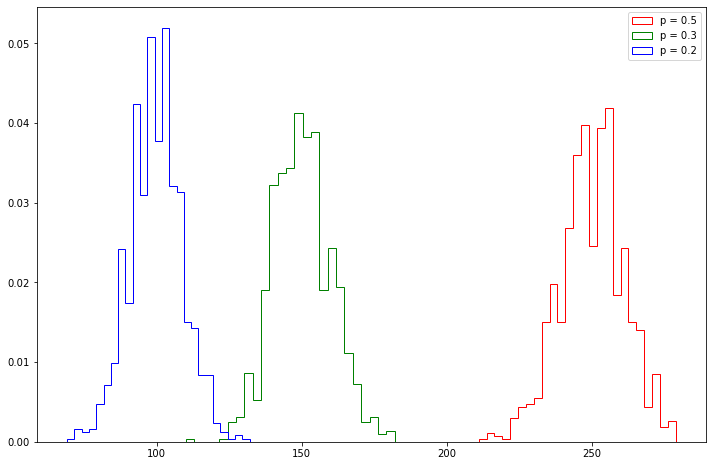
\includegraphics[width=0.9\linewidth,height=0.2\textheight,keepaspectratio]{Figure-15-01}
\end{figure}

\textbf{Exercise 15.6.5 (Computer Experiment)}. Write a function to
generate \(\text{nsim}\) observations from a Multivariate normal with
given mean \(\mu\) and covariance matrix \(\Sigma\).

\textbf{Solution}. Let's construct our samples based on samples of a
standard multivariate normal \(Z \sim N(0, I)\), by making
\(X = \mu + \Sigma^{1/2} Z\).

\begin{python}
import numpy as np

def multivariate_normal_observations(mu, sigma, nsim=1):
    mu_array = np.array(mu)
    sigma_array = np.array(sigma)
    
    assert len(mu_array.shape) == 1, "mu should be a vector"
    k = mu_array.shape[0]
    
    assert sigma_array.shape == (k, k), "sigma should be a square matrix with same length as mu"
    
    # Do the eigenvalue decomposition, then get U D^{1/2} as Sigma^{1/2}
    U, D, V = np.linalg.svd(sigma_array)
    sigma_sqrt = U @ np.diag(np.sqrt(D))
    
    # Let's write our own random normal generator for fun, rather than use np.random.normal
    # Strategy: Use Box-Muller to transform two random uniform variables in (0, 1) 
    # into two standard normals
    def random_normals(size):

        def box_muller(u1, u2):
            R = np.sqrt(-2 * np.log(u1))
            theta = 2 * np.pi * u2

            z0 = R * np.cos(theta)
            z1 = R * np.sin(theta)

            return z0, z1

        def normal_generator(uniform_generator):
            while True:
                z0, z1 = box_muller(next(uniform_generator), next(uniform_generator))
                yield z0
                yield z1

        def random_generator(batch_size):
            while True:
                for v in np.random.uniform(size=batch_size):
                    yield v

        result = np.empty(size)
        gen = normal_generator(random_generator(batch_size=min(size, 1024)))
        for i in range(size):
            result[i] = next(gen)

        return result

    def get_observation():
        z = random_normals(k)
        return mu_array + sigma_sqrt @ z
    
    return np.array([get_observation() for _ in range(nsim)])
\end{python}

\begin{python}
# Sample usage
import matplotlib.pyplot as plt

mu = [1, 3]
sigma = [[2, 1], [1, 2]]
obs = multivariate_normal_observations(mu, sigma, nsim=5000)

plt.figure(figsize=(12, 8))
plt.hexbin(obs[:, 0], obs[:, 1], cmap=plt.cm.Reds)
plt.show()
\end{python}

\begin{figure}[H]
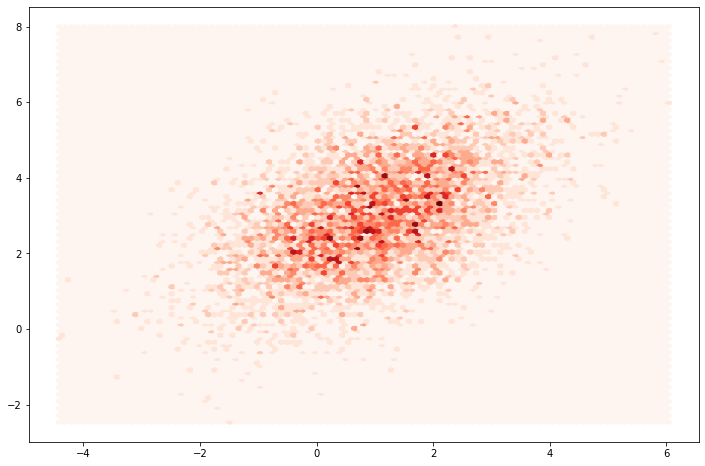
\includegraphics[width=0.9\linewidth,height=0.2\textheight,keepaspectratio]{Figure-15-02}
\end{figure}

\textbf{Exercise 15.6.6 (Computer Experiment)}. Generate 1000 random
vectors from a \(N(\mu, \Sigma)\) distribution where

\[ \mu = \begin{pmatrix} 3 \\ 8\end{pmatrix}
, \quad
\Sigma = \begin{pmatrix}
2 & 6 \\
6 & 2
\end{pmatrix}\]

Plot the simulation as a scatterplot. Find the distribution of
\(X_2 | X_1 = x_1\) using theorem 15.5. In particular, what is the
formula for \(\mathbb{E}(X_2 | X_1 = x_1)\)? Plot
\(\mathbb{E}(X_2 | X_1 = x_1)\) on your scatterplot. Find the
correlation \(\rho\) between \(X_1\) and \(X_2\). Compare this with the
sample correlations from your simulation. Find a 95\% confidence
interval for \(\rho\). Estimate the covariance matrix \(\Sigma\).

\textbf{Solution}.

The provided \(\Sigma\) matrix has negative eigenvalues. We will instead
use the following matrix:

\[ \Sigma = \begin{pmatrix} 6 & 2 \\ 2 & 6\end{pmatrix}\]

\begin{python}
# Generate 1000 vectors
mu = [3, 8]
sigma = [[2, 6], [6, 2]]
obs = multivariate_normal_observations(mu, sigma, nsim=1000)

# Using numpy to generate observations:
#obs = np.random.multivariate_normal(mu, sigma, size=1000)

# Using scipy to generate observations:
#obs = scipy.stats.multivariate_normal.rvs(mean=mu, cov=sigma, size=1000)

x, y = obs[:, 0], obs[:, 1]

# Plot scatterplot
plt.figure(figsize=(12, 8))
plt.scatter(x, y)
plt.show()
\end{python}

\begin{figure}[H]
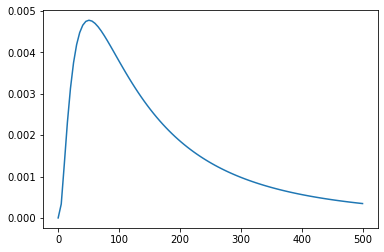
\includegraphics[width=0.9\linewidth,height=0.2\textheight,keepaspectratio]{Figure-12-04}
\end{figure}

From theorem 15.5,

\[ X_2 | X_1 = x_1 \sim N(\mu(x_1), \Sigma(x_1))\]

where

\begin{align}
\mu(x_1) &= \mu_2 + \Sigma_{21} \Sigma_{11}^{-1} (x_1 - \mu_1) \\
\Sigma(x_1) &= \Sigma_{22} - \Sigma_{21}\Sigma_{11}^{-1}\Sigma_{12}
\end{align}

Replacing the given values,

\begin{align}
\mu(x_1) &= 8 + 2 \cdot 6^{-1} (x_1 - 3) = \frac{1}{3} x_1 + \frac{22}{3}\\
\Sigma(x_1) &= 6 - 2 \cdot 6^{-1} \cdot 2 = \frac{16}{3}
\end{align}

\begin{python}
# Plot scatterplot + line
f = lambda x: x/3 + 22/3

plt.figure(figsize=(12, 8))
plt.scatter(x, y)
plt.plot([-6, 10], [f(-6), f(10)], color='red')
plt.show()
\end{python}

\begin{figure}[H]
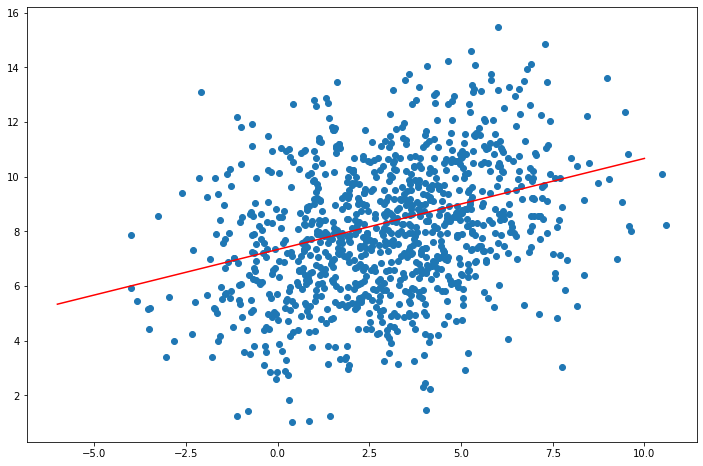
\includegraphics[width=0.9\linewidth,height=0.2\textheight,keepaspectratio]{Figure-15-04}
\end{figure}

The correlation \(\rho\) between \(X_1\) and \(X_2\) is:

\[ \rho = \frac{\text{Cov}(X_1, X_2)}{\sigma_{X_1} \sigma_{X_2}} = \frac{1}{3}\]

The estimated correlation \(\rho\) between \(X_1\) and \(X_2\) is:

\[ \hat{\rho} = \frac{\sum_i (X_{1i} - \overline{X}_1)(X_{2i} - \overline{X}_2)}{s_{X_1} s_{X_2}}\]

\begin{python}
rho_hat = np.corrcoef(x, y)[0, 1]
print("Estimated correlation: %.3f" % rho_hat)
\end{python}

\begin{console}
Estimated correlation: 0.327
\end{console}

We will use the provided process to estimate a confidence interval for
the correlation:

\textbf{Approximate Confidence Interval for the Correlation}

\begin{enumerate}[tightlist,label={\arabic*.}]
\item
  Compute
\end{enumerate}

\[\hat{\theta} = f(\hat{\rho}) = \frac{1}{2} \left( \log(1 + \hat{\rho}) - \log(1 - \hat{\rho})\right) \]

\begin{enumerate}[tightlist,label={\arabic*.},resume]
\item
  Compute the approximate standard error of \(\hat{\theta}\) which can
  be shown to be
\end{enumerate}

\[\hat{\text{se}}(\hat{\theta}) = \frac{1}{\sqrt{n - 3}} \]

\begin{enumerate}[tightlist,label={\arabic*.},resume]
\item
  An approximate \(1 - \alpha\) confidence interval for
  \(\theta = f(\rho)\) is
\end{enumerate}

\[(a, b) \equiv \left(\hat{\theta} - \frac{z_{\alpha/2}}{\sqrt{n - 3}}, \; \hat{\theta} + \frac{z_{\alpha/2}}{\sqrt{n - 3}} \right)\]

\begin{enumerate}[tightlist,label={\arabic*.},resume]
\item
  Apply the inverse transformation \(f^{-1}(z)\) to get a confidence
  interval for \(\rho\):
\end{enumerate}

\[ \left( \frac{e^{2a} - 1}{e^{2a} + 1}, \frac{e^{2b} - 1}{e^{2b} + 1} \right) \]

\begin{python}
from scipy.stats import norm

theta_hat = (np.log(1 + rho_hat) - np.log(1 - rho_hat)) / 2
se_theta_hat = 1 / np.sqrt(1000 - 3)
z = norm.ppf(0.975)
a, b = theta_hat - z * se_theta_hat, theta_hat + z * se_theta_hat
f_inv = lambda x: (np.exp(2*x) - 1) / (np.exp(2*x) + 1)
confidence_interval = (f_inv(a), f_inv(b))

print('95%% confidence interval: %.3f, %.3f' % confidence_interval)
\end{python}

\begin{console}
95\% confidence interval: 0.270, 0.381
\end{console}

The sample covariance matrix is:

\[ \hat{\Sigma} = \frac{1}{n} S = \frac{1}{n} \sum_{i=1}^n (X_i - \overline{X})(X_i - \overline{X})^T \]

\begin{python}
import numpy as np
mu_hat = np.array([x.mean(), y.mean()])
xx = np.concatenate((x.reshape(-1, 1), y.reshape(-1, 1)), axis=1)
sigma_hat = (xx - mu_hat).T @ (xx - mu_hat) / 1000

sigma_hat
\end{python}

\begin{console}
array([[6.17974344, 1.99813879],
       [1.99813879, 6.05196861]])
\end{console}

\textbf{Exercise 15.6.7 (Computer Experiment)}. Generate 100 random
vectors from a multivariate Normal with mean \((0, 2)^T\) and variance

\[ \begin{pmatrix}
1 & 3 \\
3 & 1
\end{pmatrix} \]

Find a 95\% confidence interval for the correlation \(\rho\). What is
the true value of \(\rho\)?

\textbf{Solution}.

The provided matrix, yet again, has negative eigenvalues. Let's instead
use:

\[\Sigma = \begin{pmatrix}
3 & 1 \\
1 & 3
\end{pmatrix}\]

\begin{python}
# Generate 100 vectors
n = 100
mu = [0, 2]
sigma = [[3, 1], [1, 3]]
obs = multivariate_normal_observations(mu, sigma, nsim=n)
x, y = obs[:, 0], obs[:, 1]
\end{python}

\begin{python}
# Find 95% confidence interval
from scipy.stats import norm

rho_hat = np.corrcoef(x, y)[0, 1]
theta_hat = (np.log(1 + rho_hat) - np.log(1 - rho_hat)) / 2
se_theta_hat = 1 / np.sqrt(n - 3)
z = norm.ppf(0.975)
a, b = theta_hat - z * se_theta_hat, theta_hat + z * se_theta_hat
f_inv = lambda x: (np.exp(2*x) - 1) / (np.exp(2*x) + 1)
confidence_interval = (f_inv(a), f_inv(b))

print('95%% confidence interval: %.3f, %.3f' % confidence_interval)
\end{python}


\begin{console}
95\% confidence interval: 0.054, 0.424
\end{console}

True value of \(\rho\):

\[ \rho = \frac{\text{Cov}(X_1, X_2)}{\sigma_{X_1} \sigma_{X_2}} = \frac{1}{3}\]
